% TODO uploudovat posledni verzi domenoveho modelu
\chapter{Doménový model před úpravami}\label{dodatek:DomainModel}
    \begin{figure}\centering
	    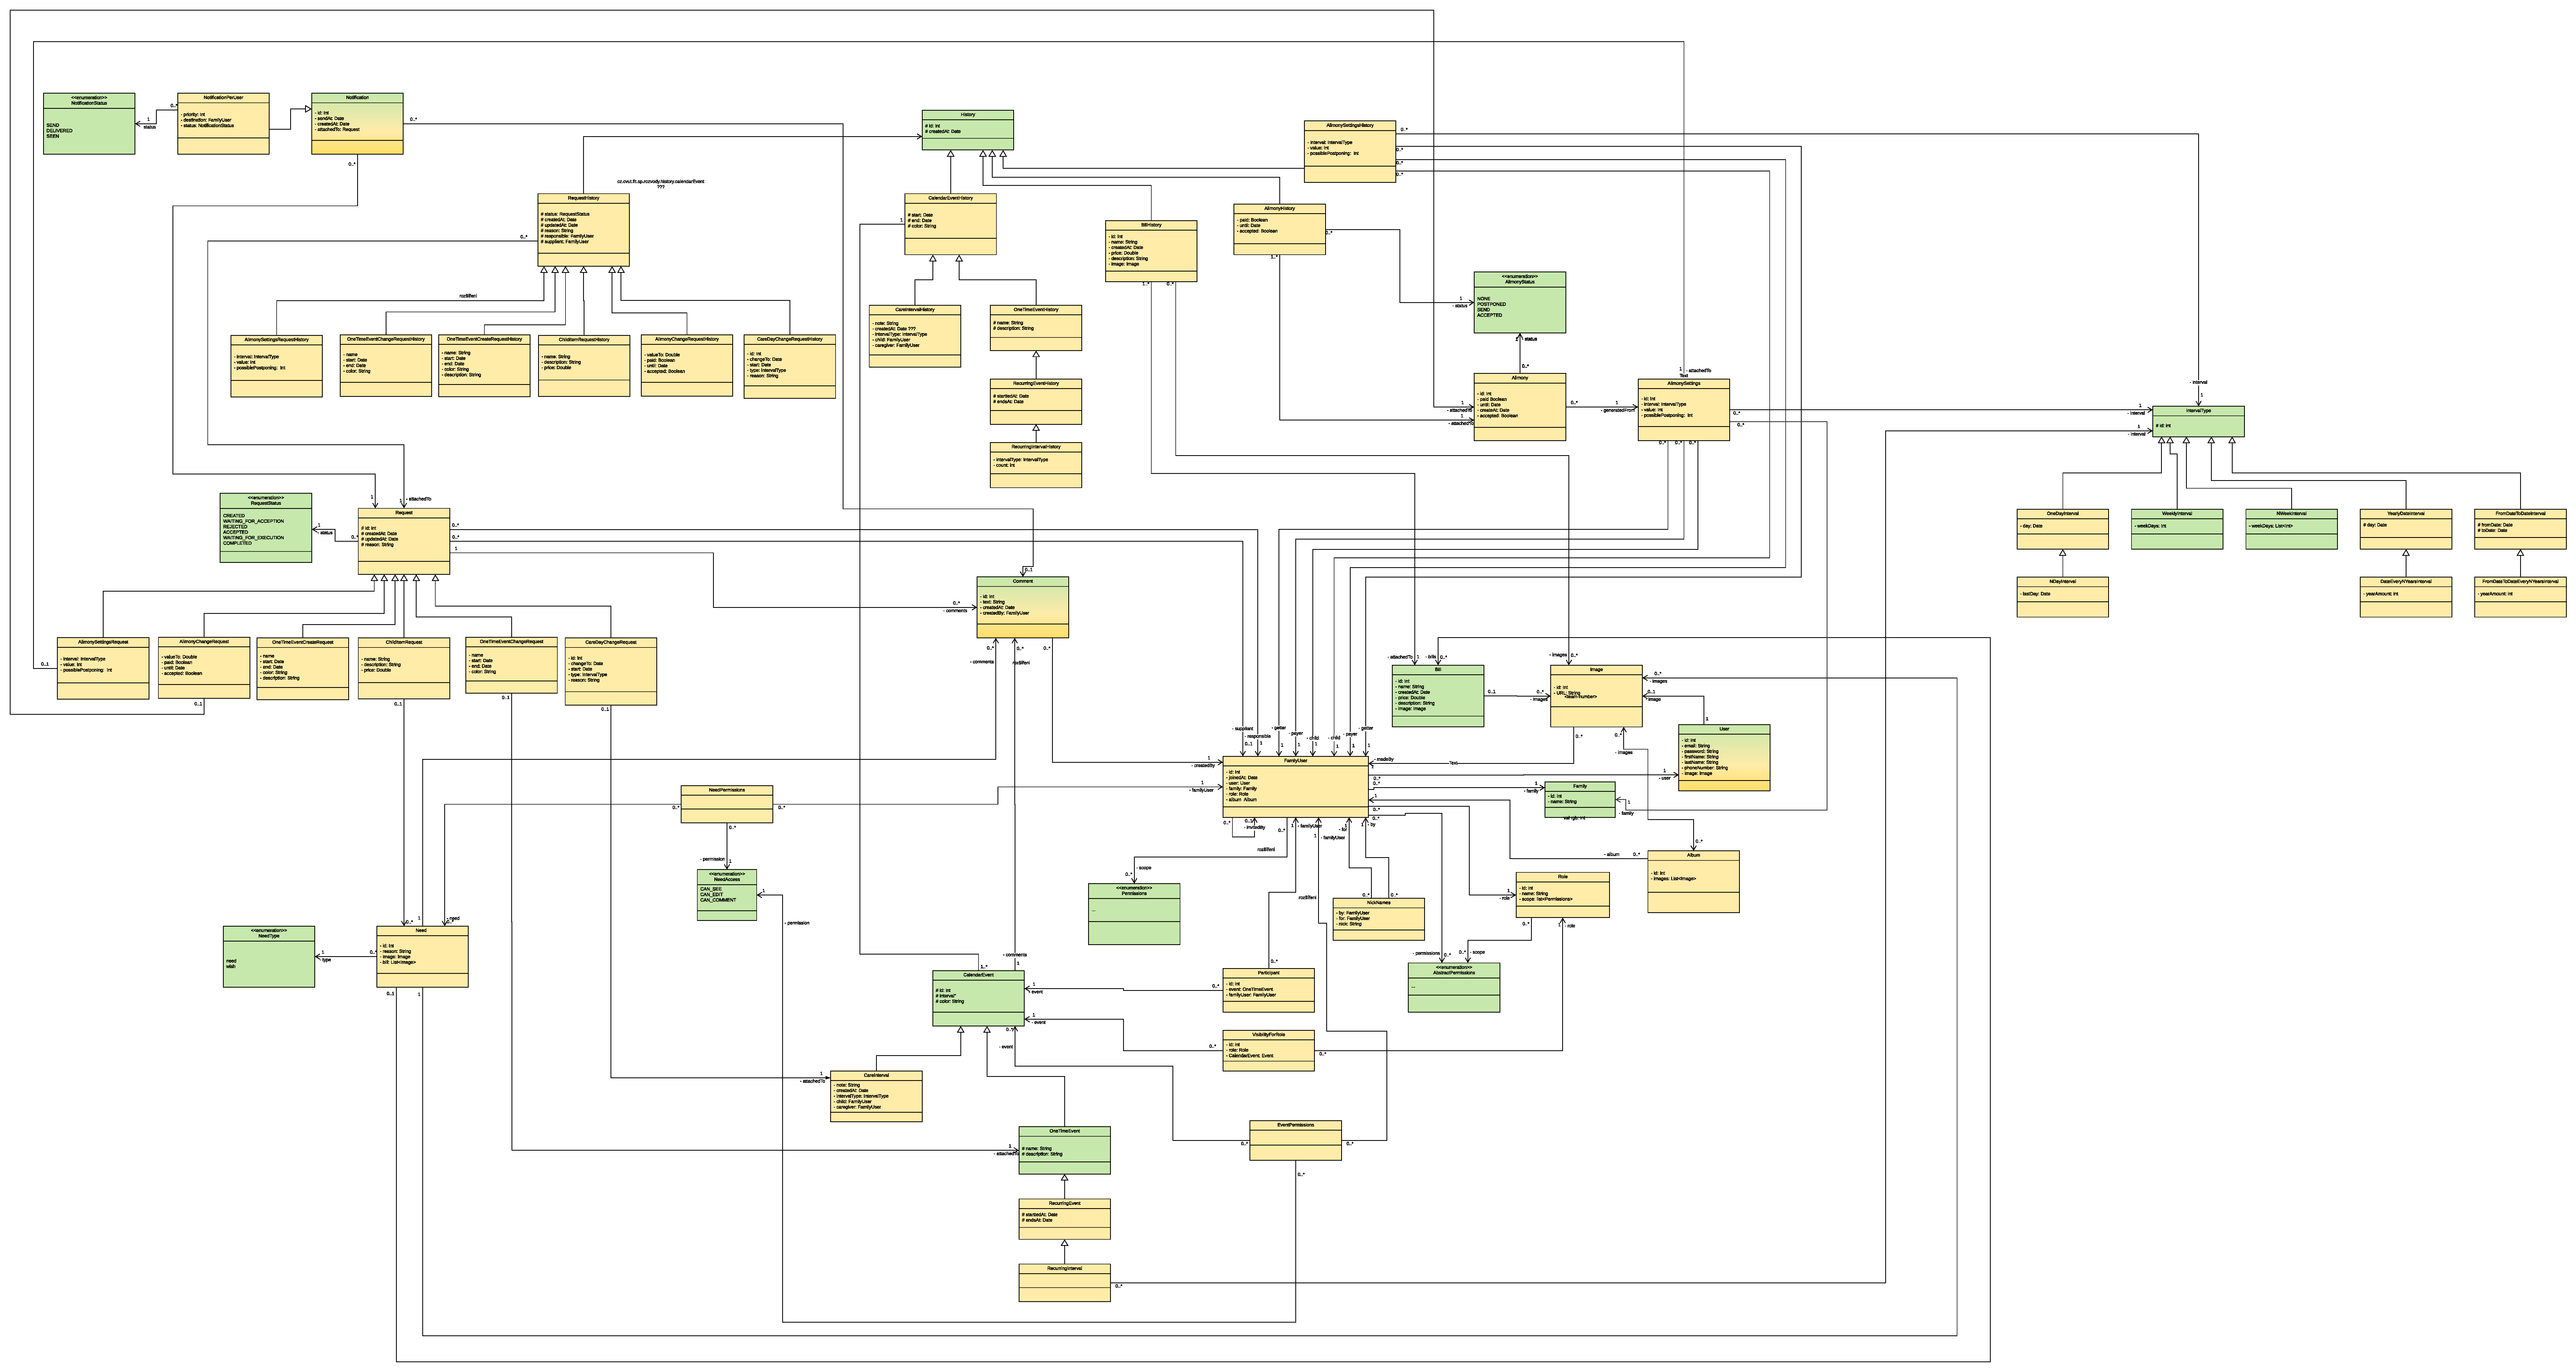
\includegraphics[angle=90, height=1.0\textheight]{pdfs/Domain-Model}
	    \caption[Doménový model před úpravami]{Doménový model z předmětu BI-SP2}\label{image:DomainModel}
    \end{figure}

\chapter{Testování}\label{dodatek:testing}
% \chapter{Pokrytí kódů testy}\label{dodatek:code-coverage}
    \begin{figure}\centering
	    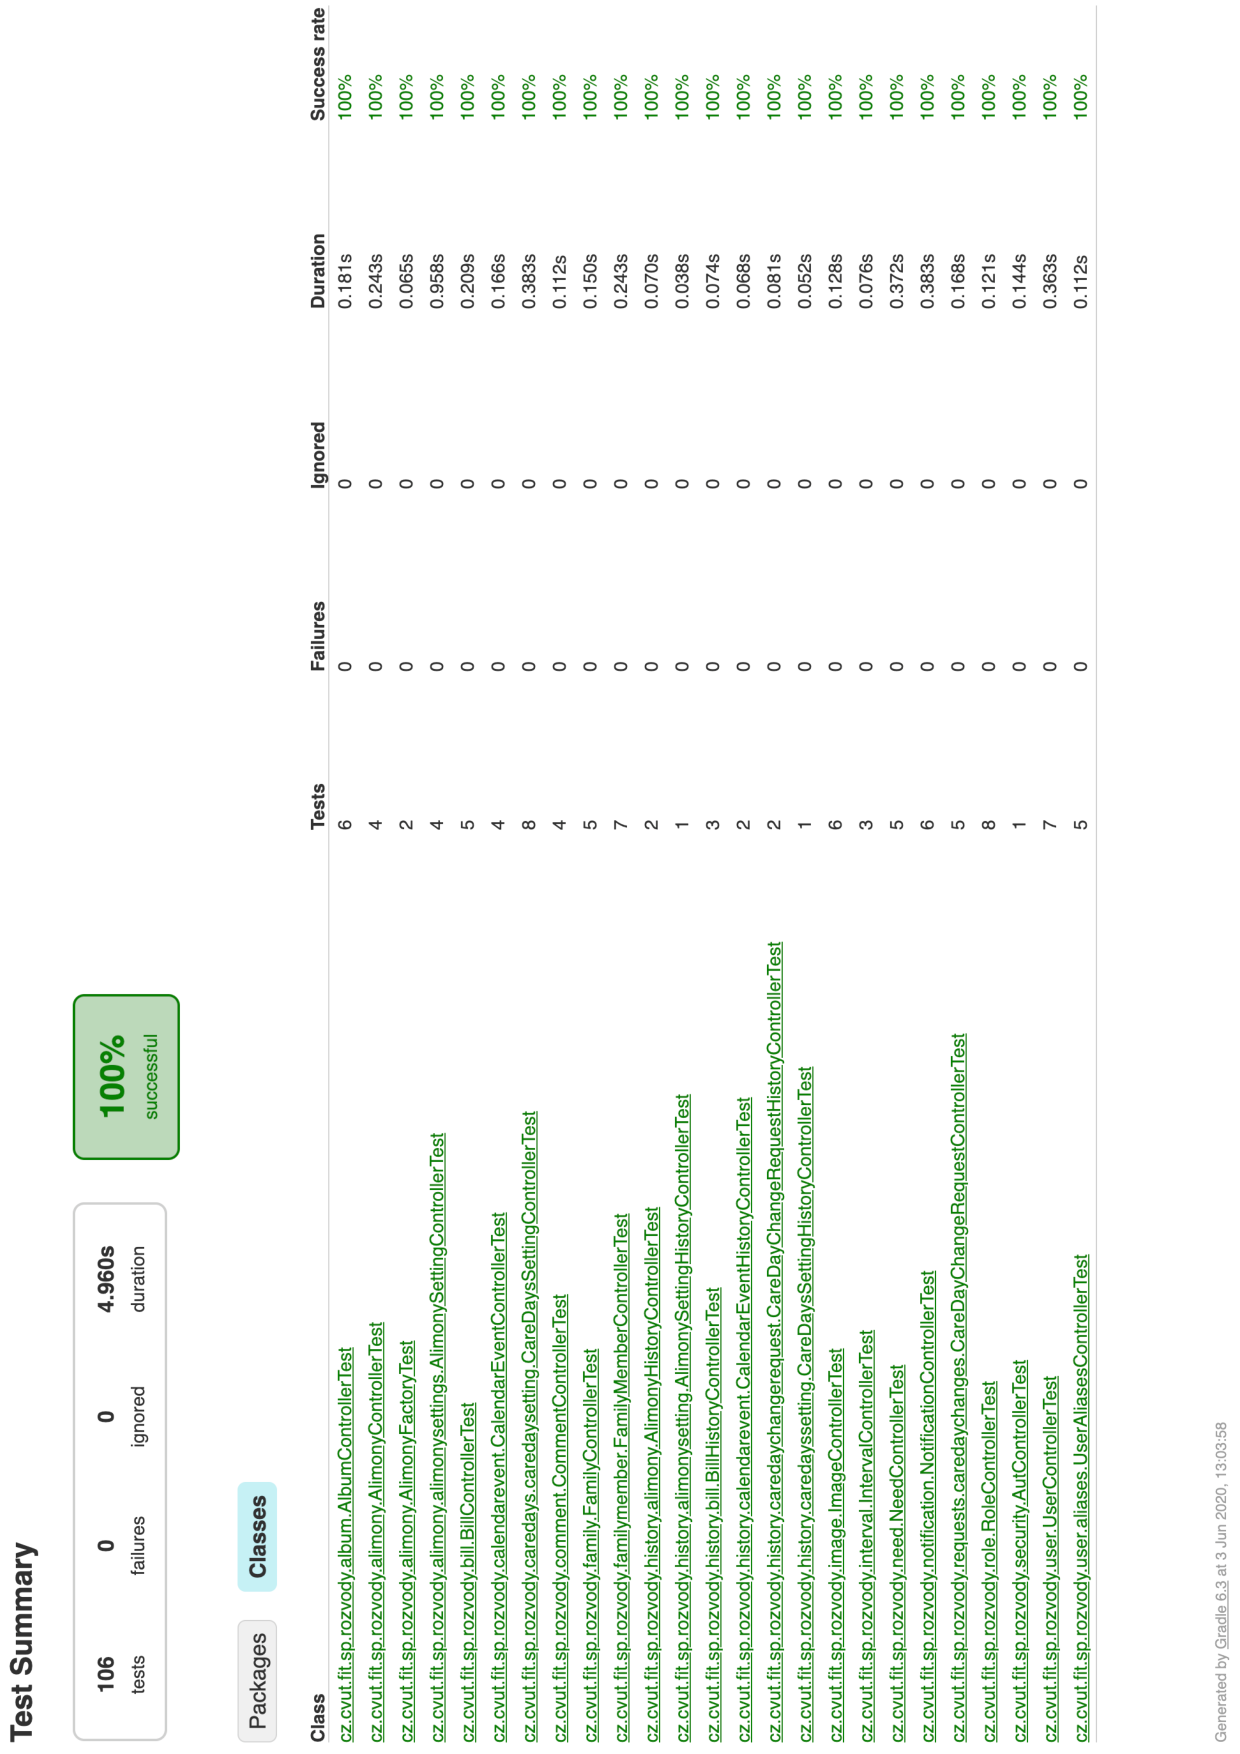
\includegraphics[width=1.0\textwidth]{pdfs/Gradle-unit-tests}
	    \caption[Seznam tříd obsahujících unit testy]{Seznam tříd obsahujících unit testy vygenerovaný pomocí nástroje Gradle}\label{image:gradle-unit-tests}
    \end{figure}
    \begin{figure}\centering
	    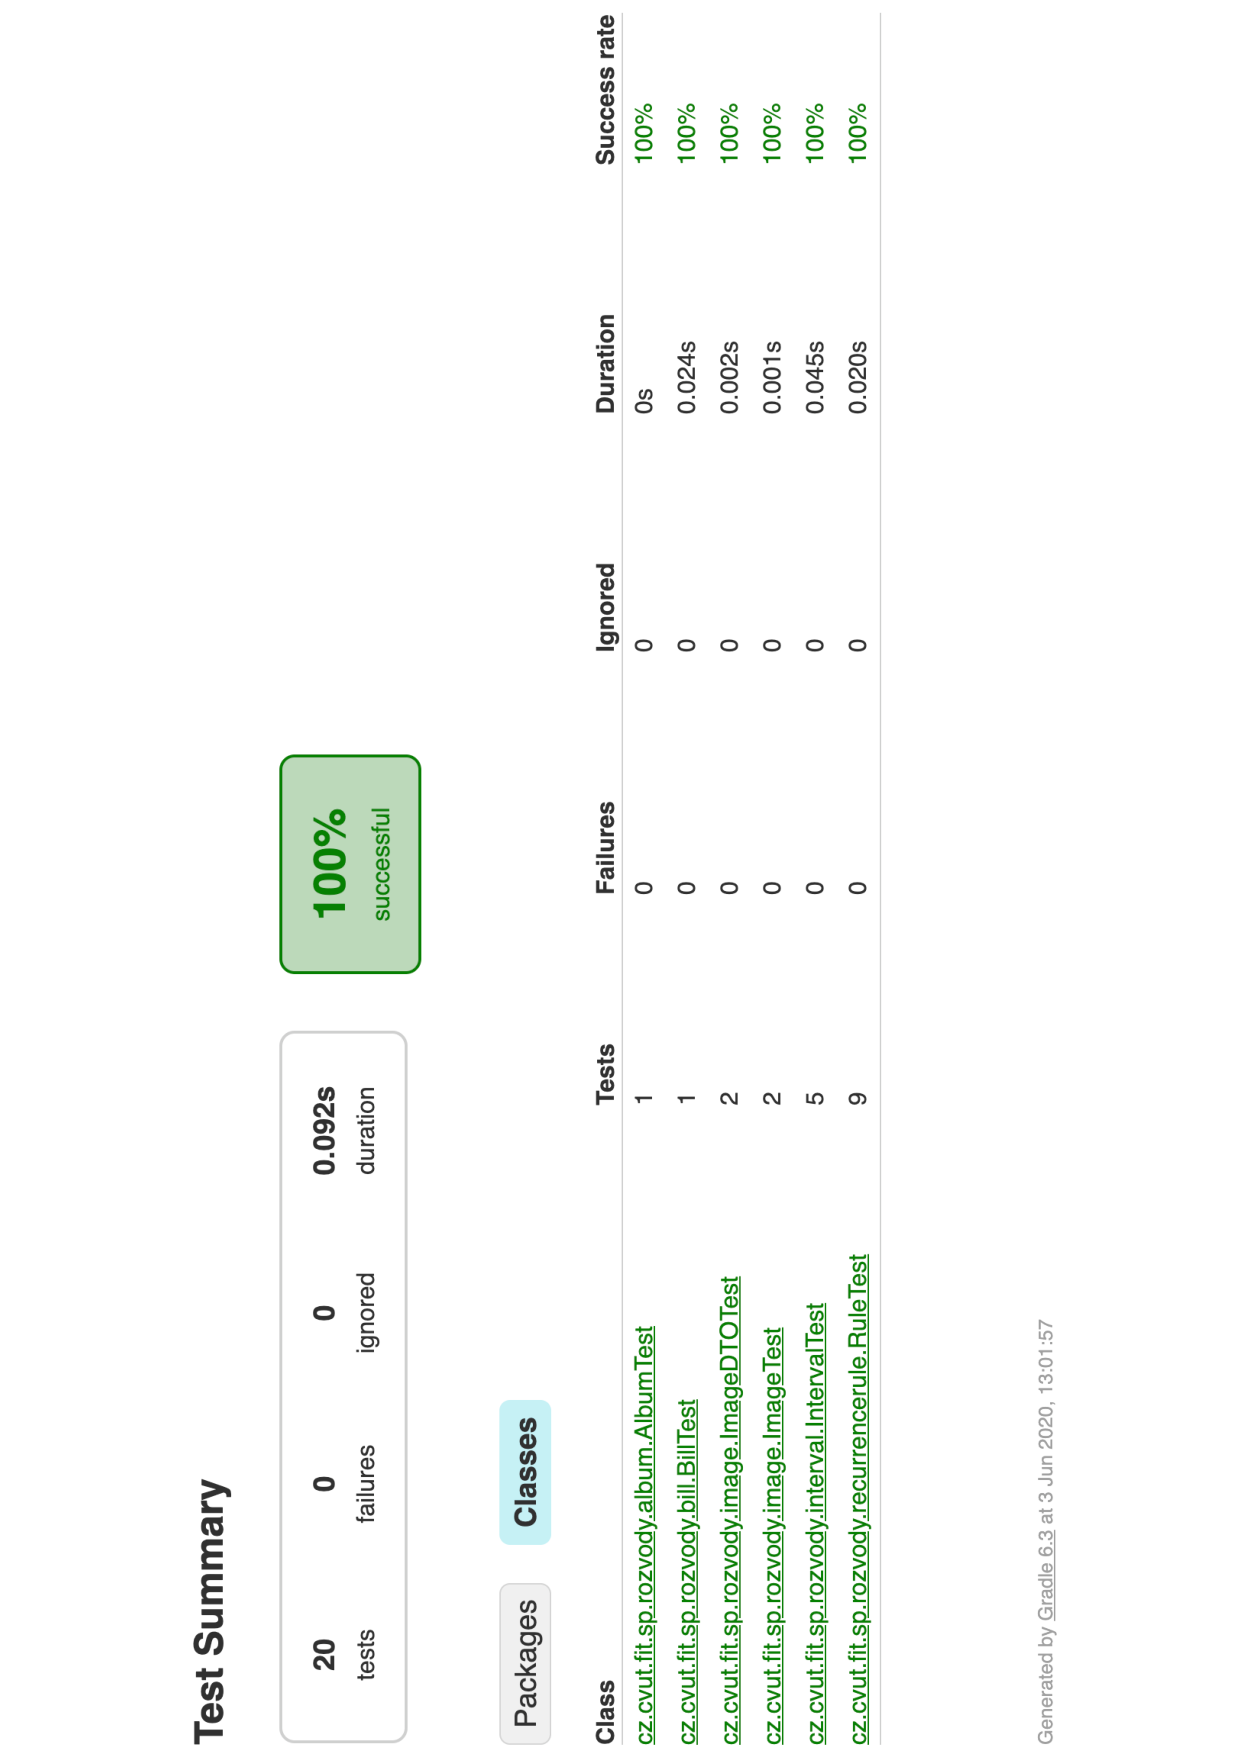
\includegraphics[width=1.0\textwidth]{pdfs/Gradle-integration-tests}
	    \caption[Seznam tříd obsahujících integrační testy]{Seznam tříd obsahující integračních testy vygenerovaný pomocí nástroje Gradle}\label{image:gradle-integration-tests}
    \end{figure}
    \begin{figure}\centering
	    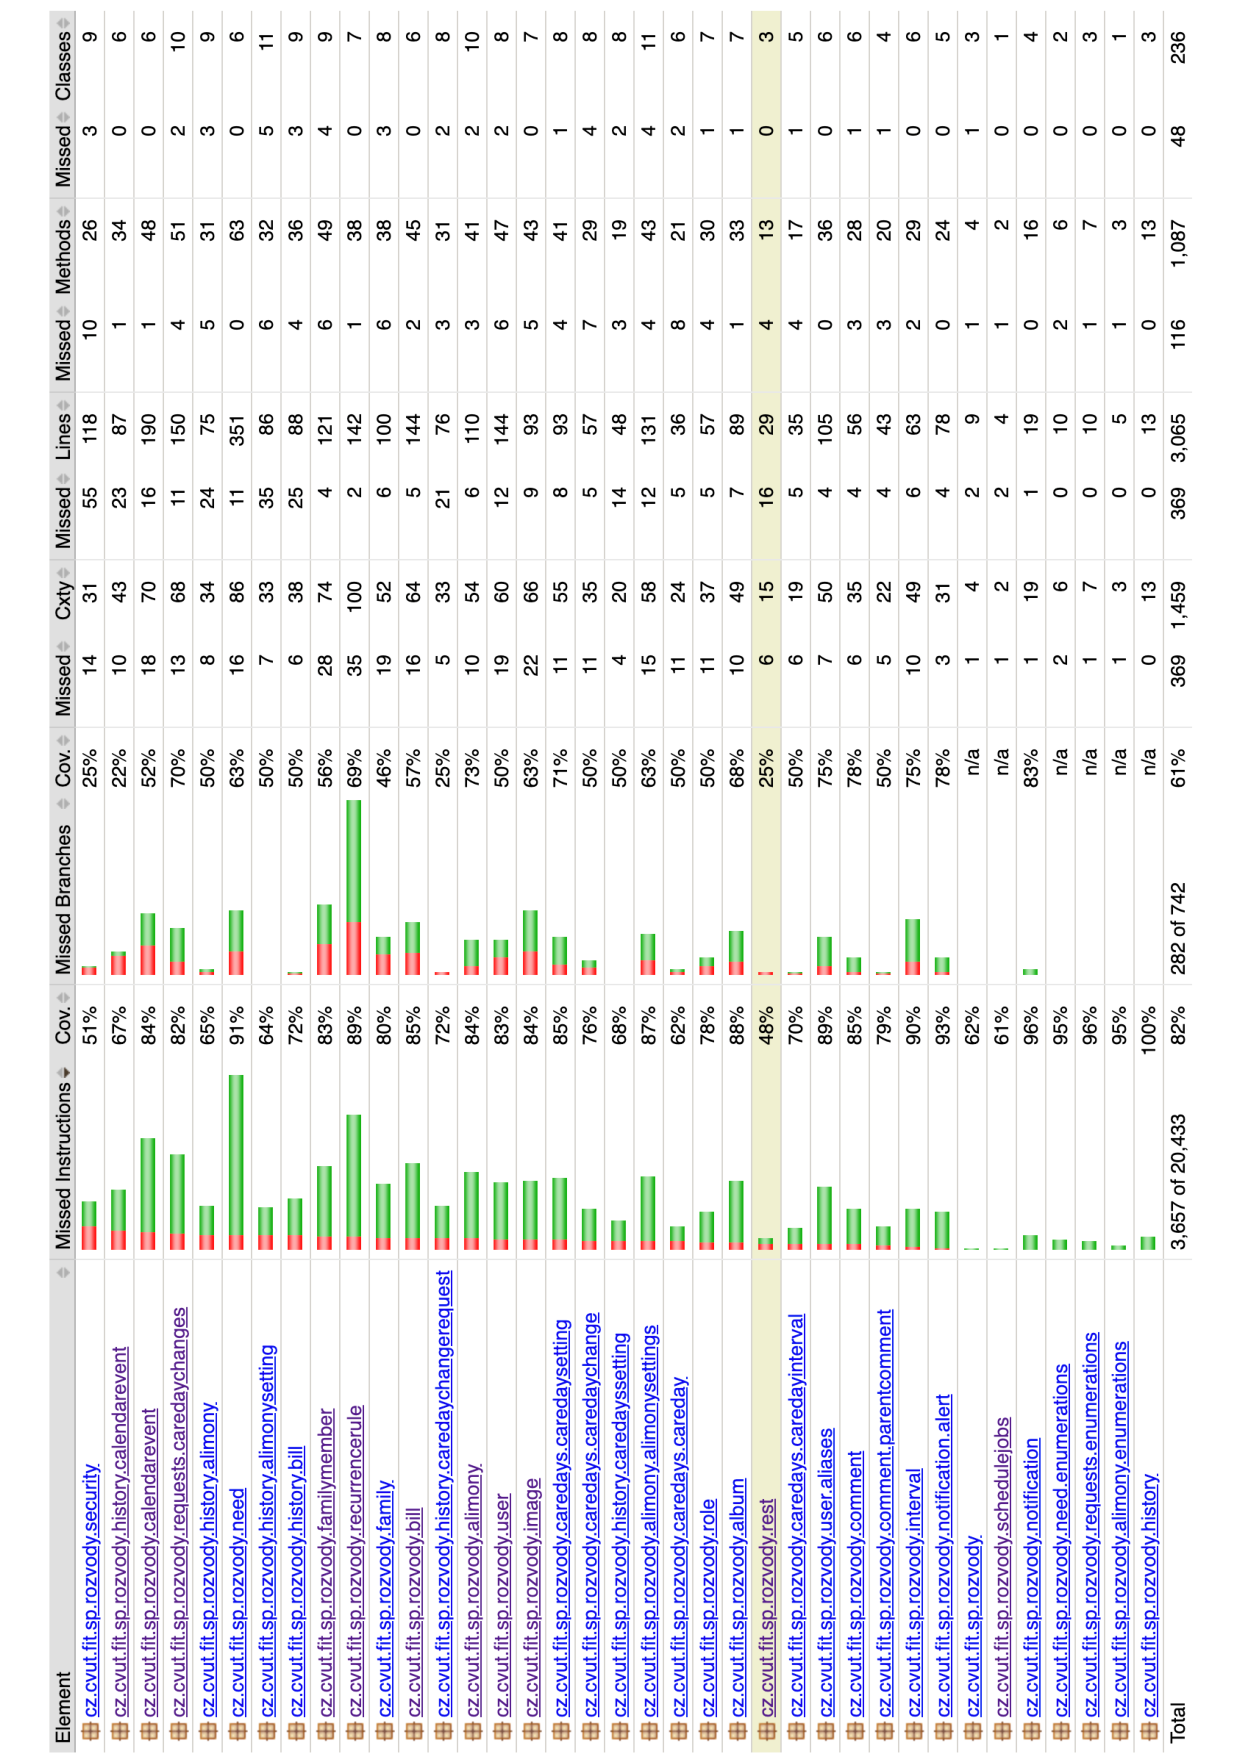
\includegraphics[width=1.0\textwidth]{pdfs/JaCoCo-results}
	    \caption[Pokrytí kódů testy podle JaCoCo]{Poslední verze výsledku pokrytí kódů testy podle JaCoCo}\label{image:jacoco-results}
    \end{figure}
    \begin{figure}\centering
	    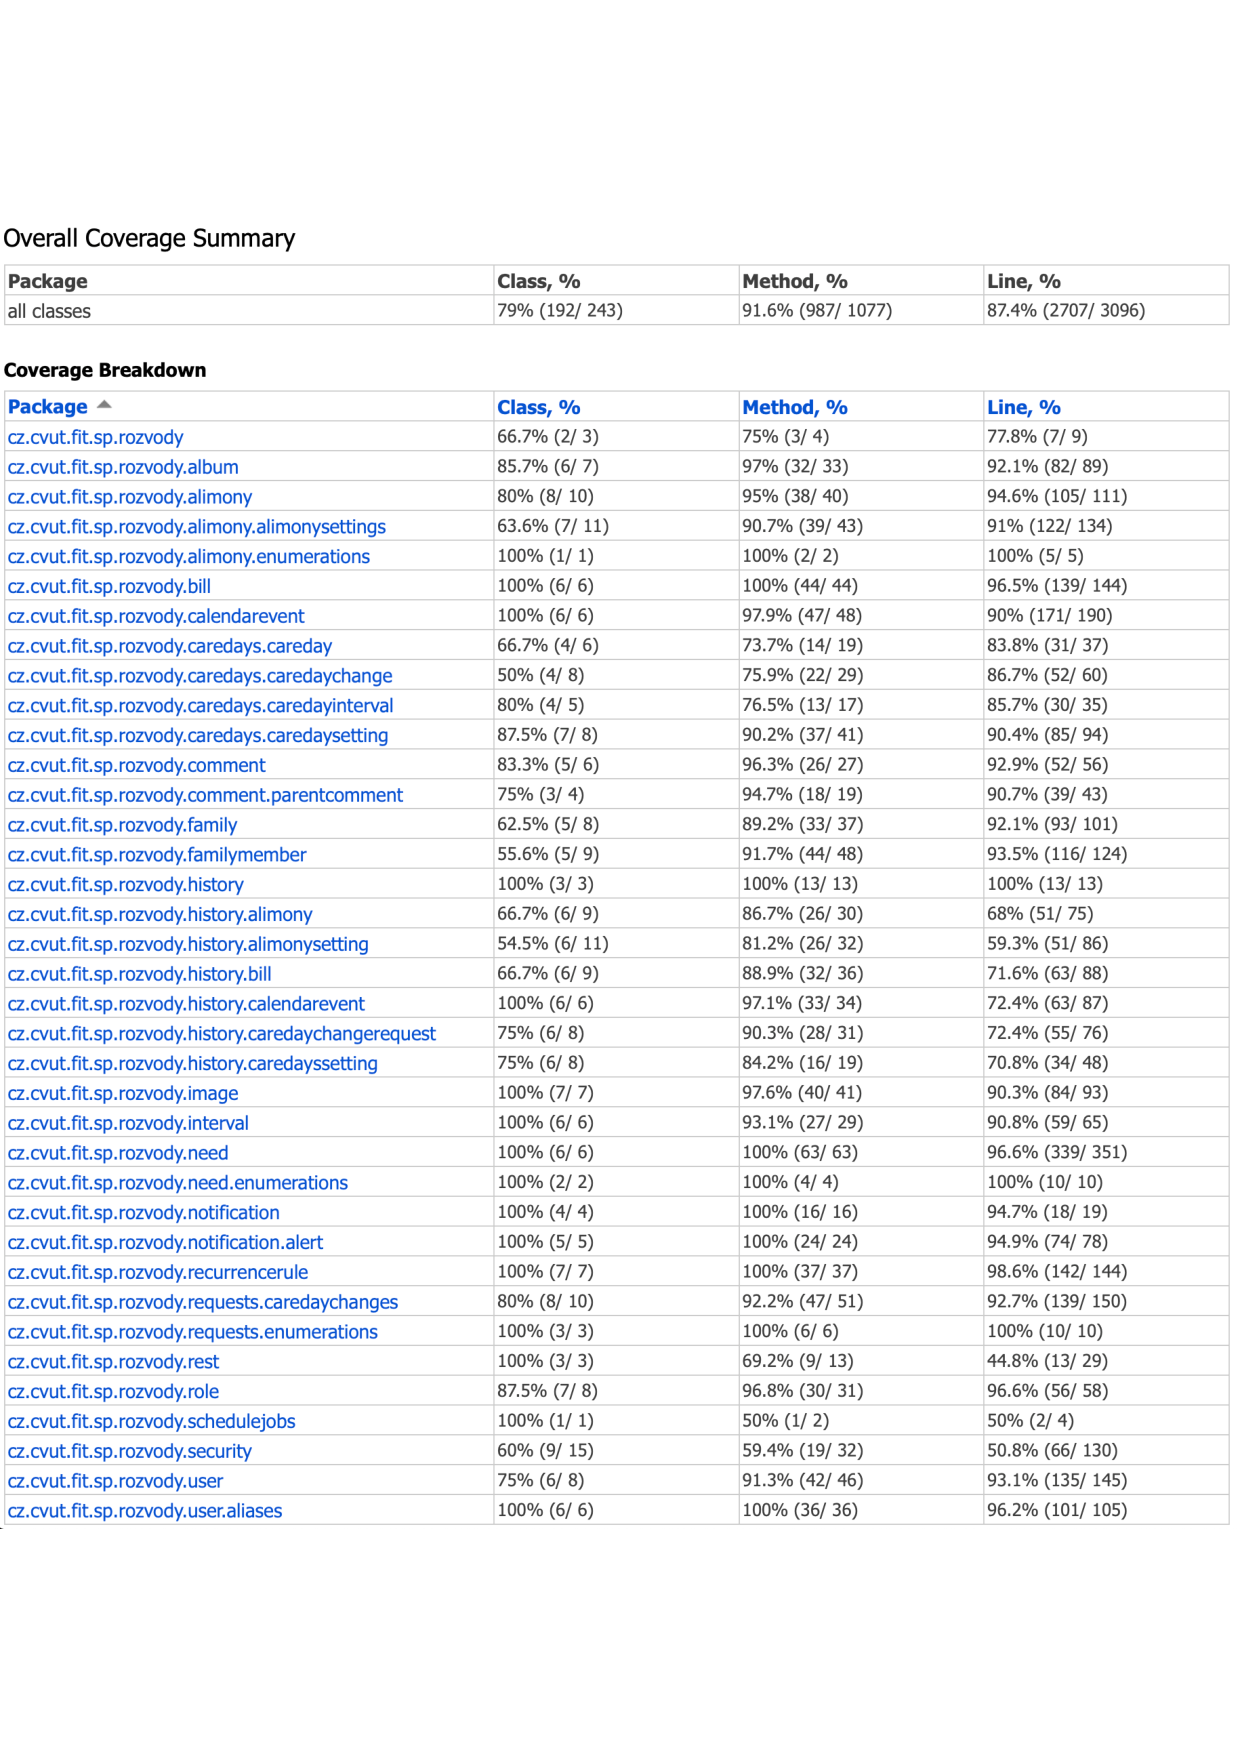
\includegraphics[width=1.0\textwidth]{pdfs/IntelliJ-IDEA-coverage-runner-results}
	    \caption[Pokrytí kódů testy podle JaCoCo]{Poslední verze výsledku pokrytí kódů testy podle IntelliJ IDEA}\label{image:intellij-coverage-result}
    \end{figure}
% TODO tady by měl být výsledný Domenový model
\chapter{Výsledný doménový model}\label{dodatek:DomainModel2}
    \begin{figure}\centering
	    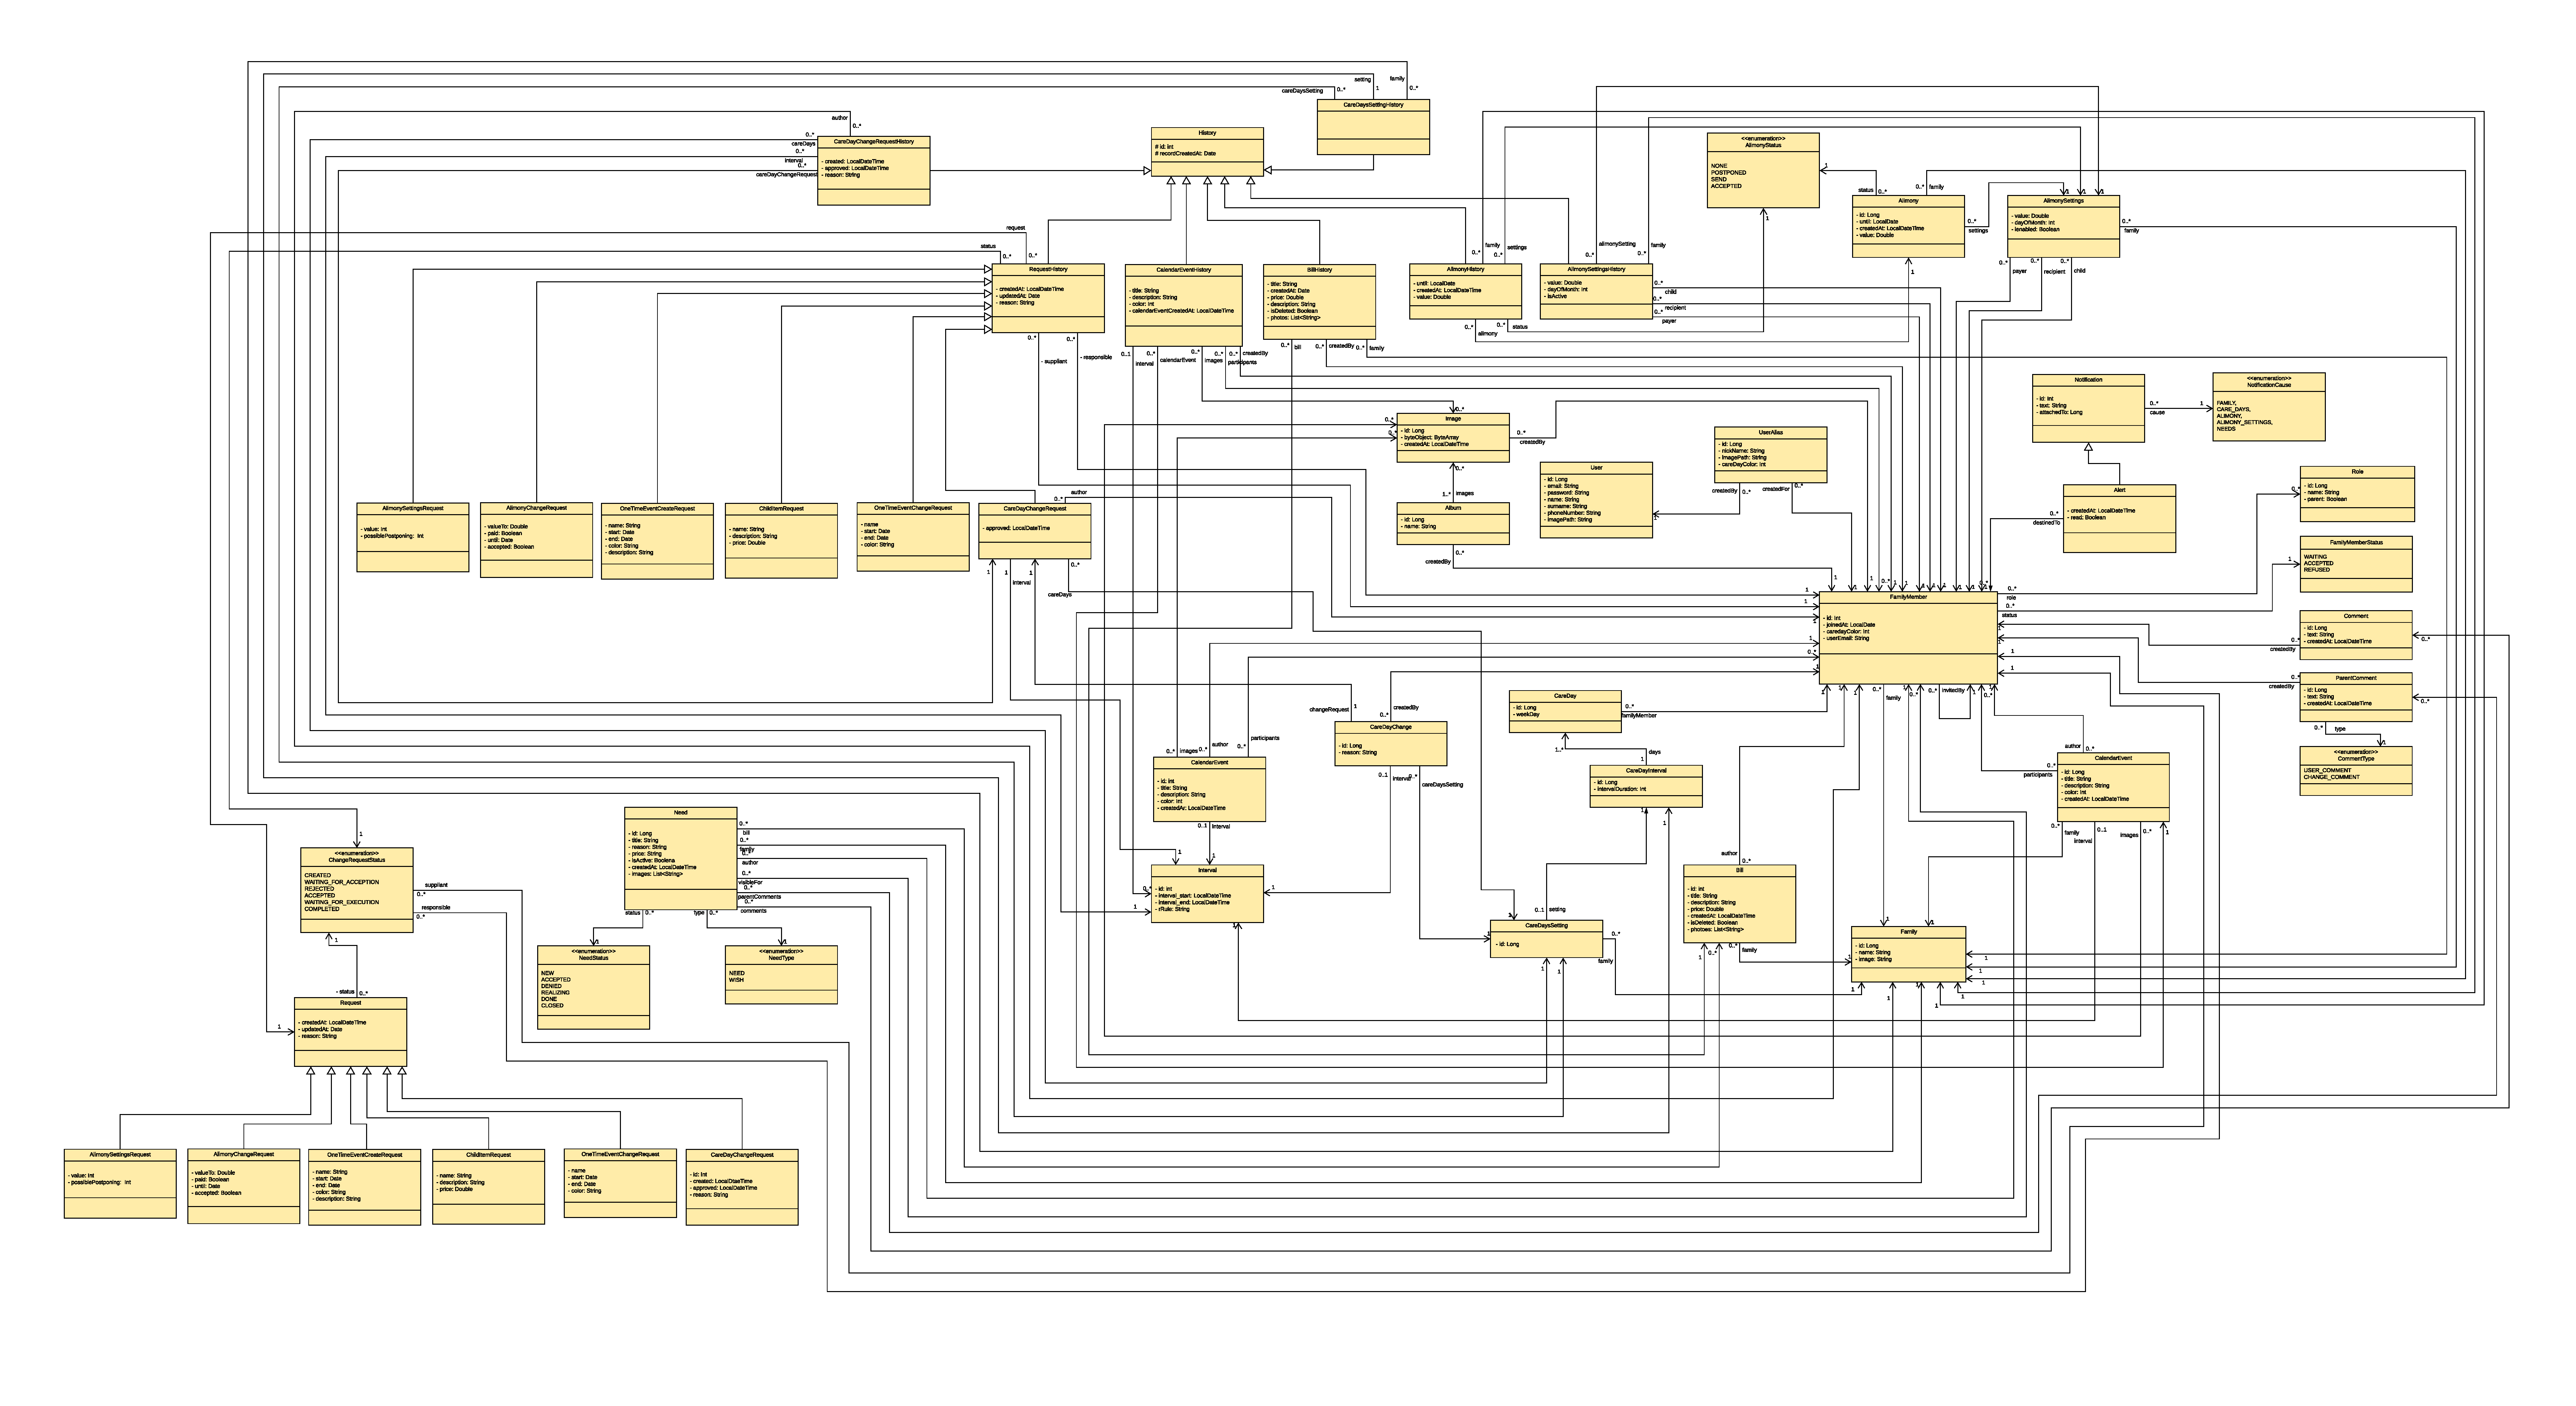
\includegraphics[angle=90, height=1.0\textheight]{pdfs/DomainModel2}
	    \caption[Výsledný doménový model]{Doménový model po navržení a implementaci všech úprav}\label{image:DomainModel2}
    \end{figure}
\chapter{Konfigurace výsledného našeptávače pro chyby}\label{dodatek:excpetion-handler2}
    % \begin{sidewaystable} \centering
    \begin{figure} \centering

    \begin{adjustbox}{angle=90} \centering
            \begin{tabular}{|l|c|c|c|}\hline
        	  Typ chyby		& HTTP status		& zpáva	& URL 	\tabularnewline \hline \hline
        	  \texttt{IllegalAccessException}	& 401	& původní zpráva chyby		& původní cesta     \tabularnewline \hline
        	  \texttt{IllegalArgumentException}	& 400	& původní zpráva chyby		& původní cesta     \tabularnewline \hline
        	  \texttt{NullPointerException}	& 500	& nic		& původní cesta     \tabularnewline \hline
        	  \texttt{No Such Element}	& 404	& nic		& nic     \tabularnewline \hline
        	  \texttt{MissingKotlinParameterException}	& 400	& původní zpráva chyby		& původní cesta     \tabularnewline \hline
            \end{tabular}
    % \end{sidewaystable}
    \end{adjustbox} \caption[Konfigurace výsledného našeptávače pro řadiče]{Ukázka výsledné konfigurace našeptávače zachycování výjimek pro řadiče}
    \end{figure}
\chapter{Obrázky}\label{dodatek:images}
    % ANALYZA
    \begin{figure}\centering
        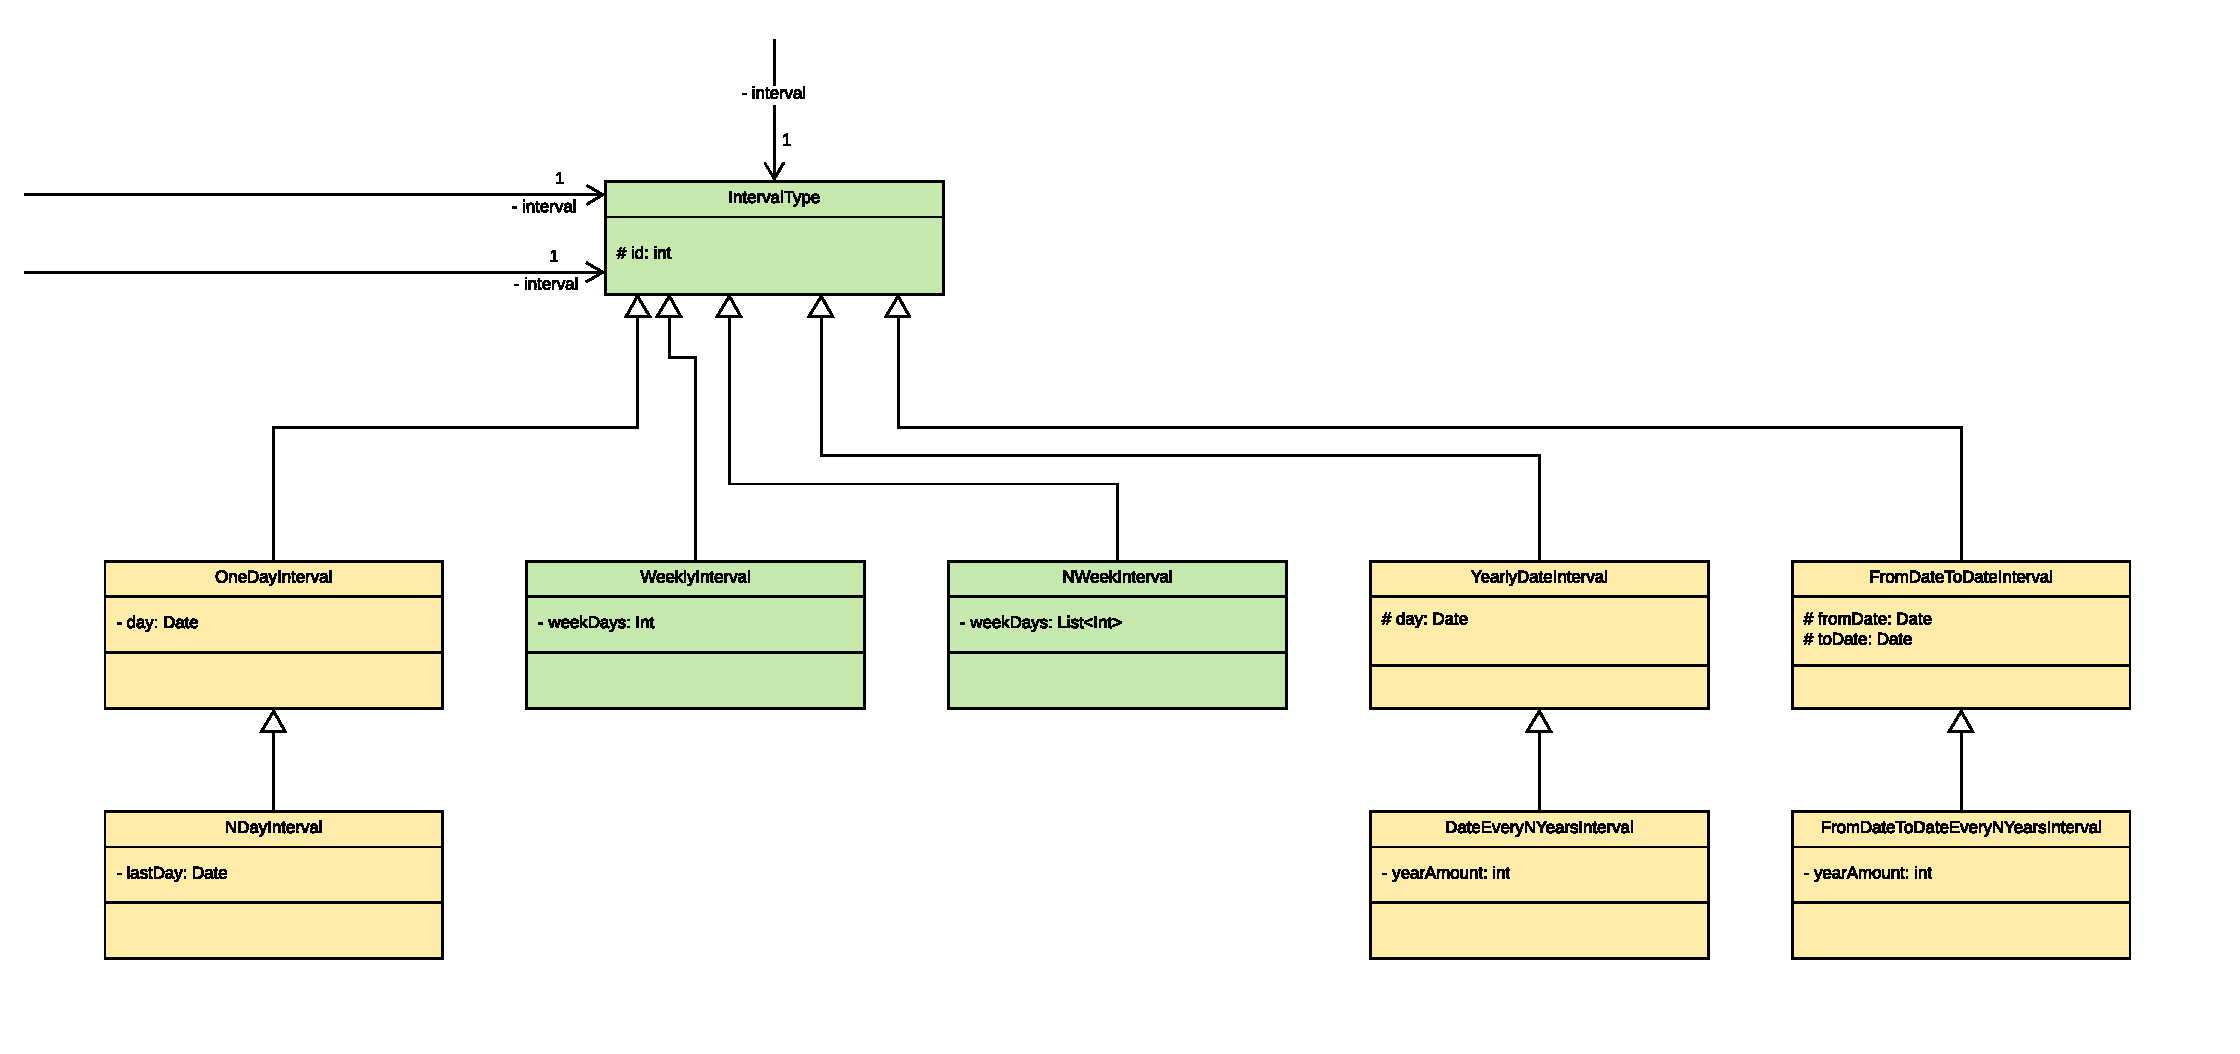
\includegraphics[angle=90, height=1.0\textheight]{pdfs/Interval1}
        \caption[Předešlý návrh entity \texttt{Interval}]{Návrh entity \textit{Interval} podle doménovém modelu z předmětu BI-SP2}\label{image:Interval1}
    \end{figure}
    \begin{figure}\centering
            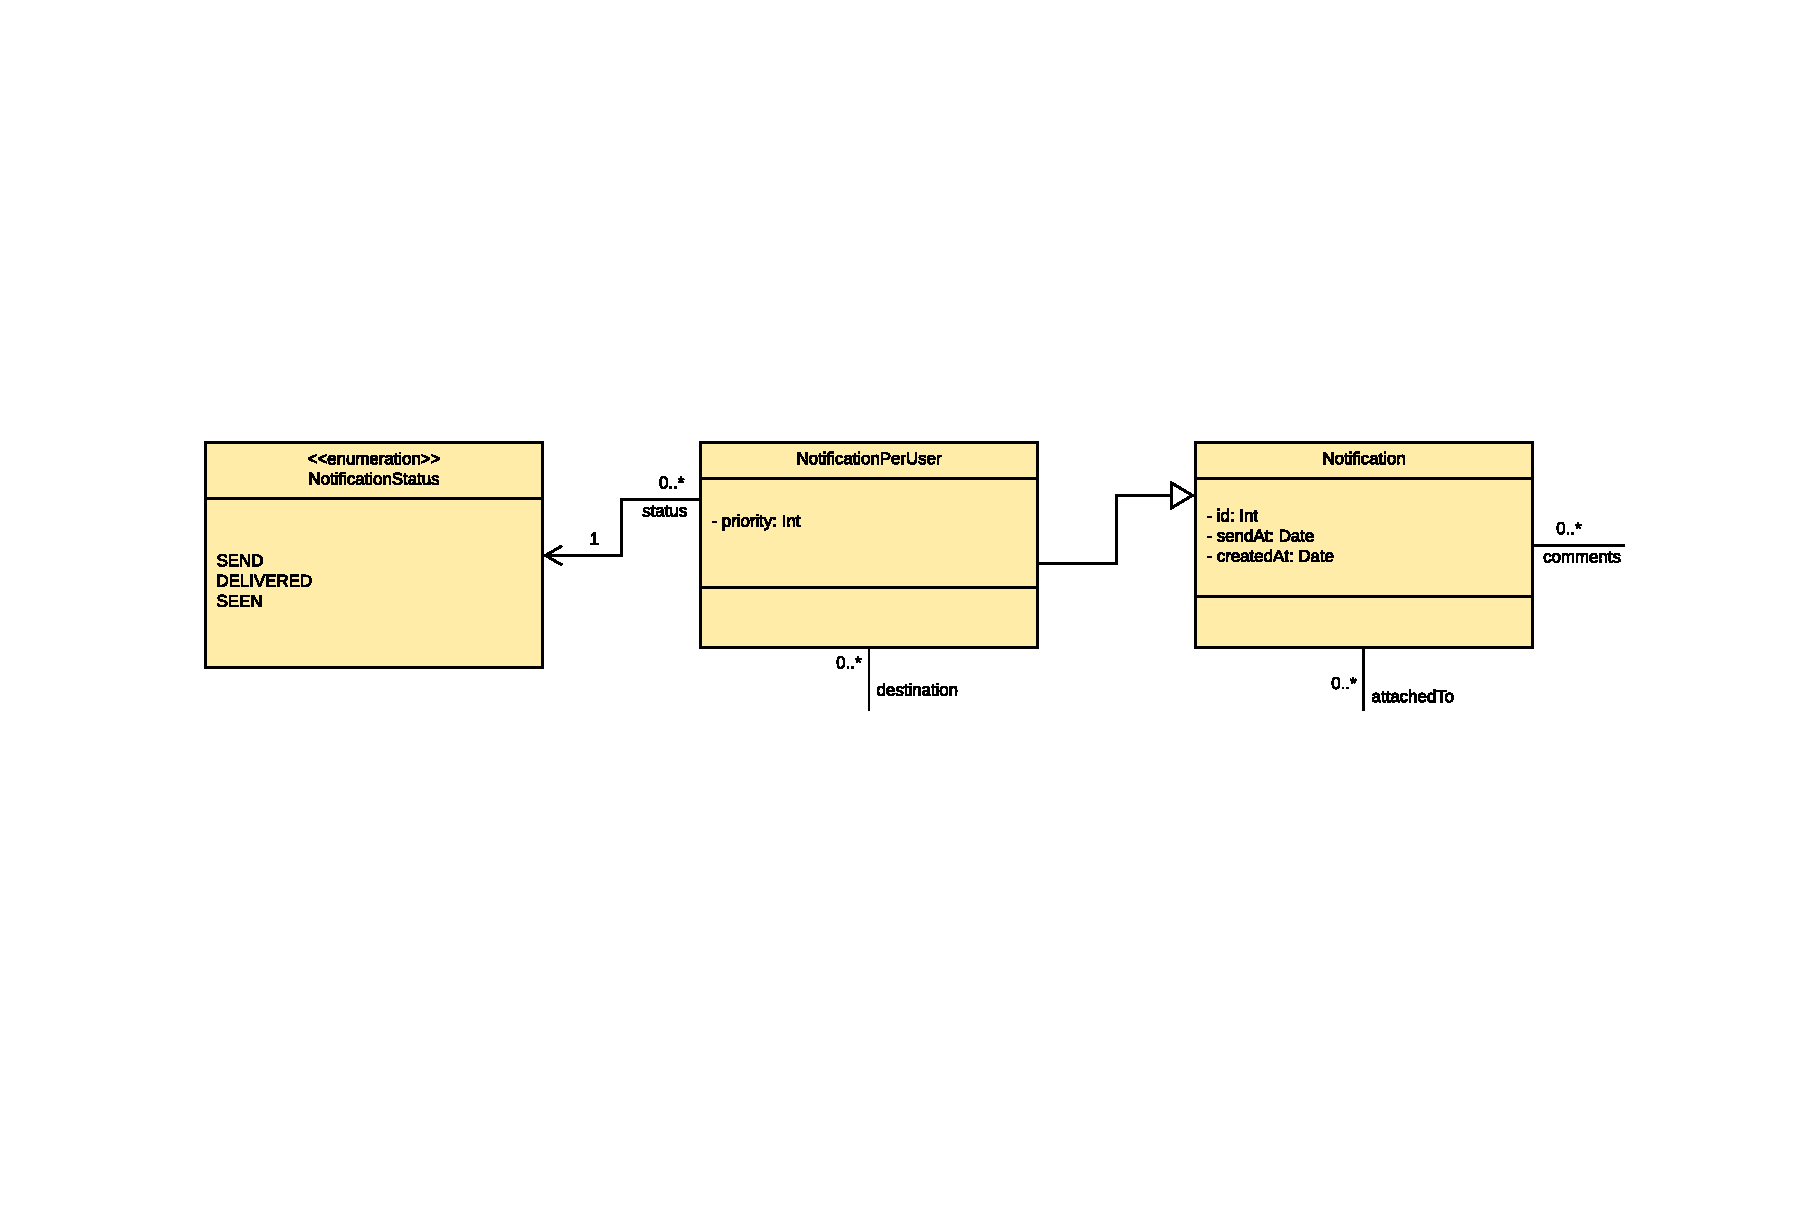
\includegraphics[angle=90, height=1.0\textheight]{pdfs/Notification1}
            \caption[Předešlý návrh oznámení]{Návrh oznámení podle doménového modelu předmětu BI-SP2}\label{image:notification1}
        \end{figure}
        \begin{figure}\centering
	        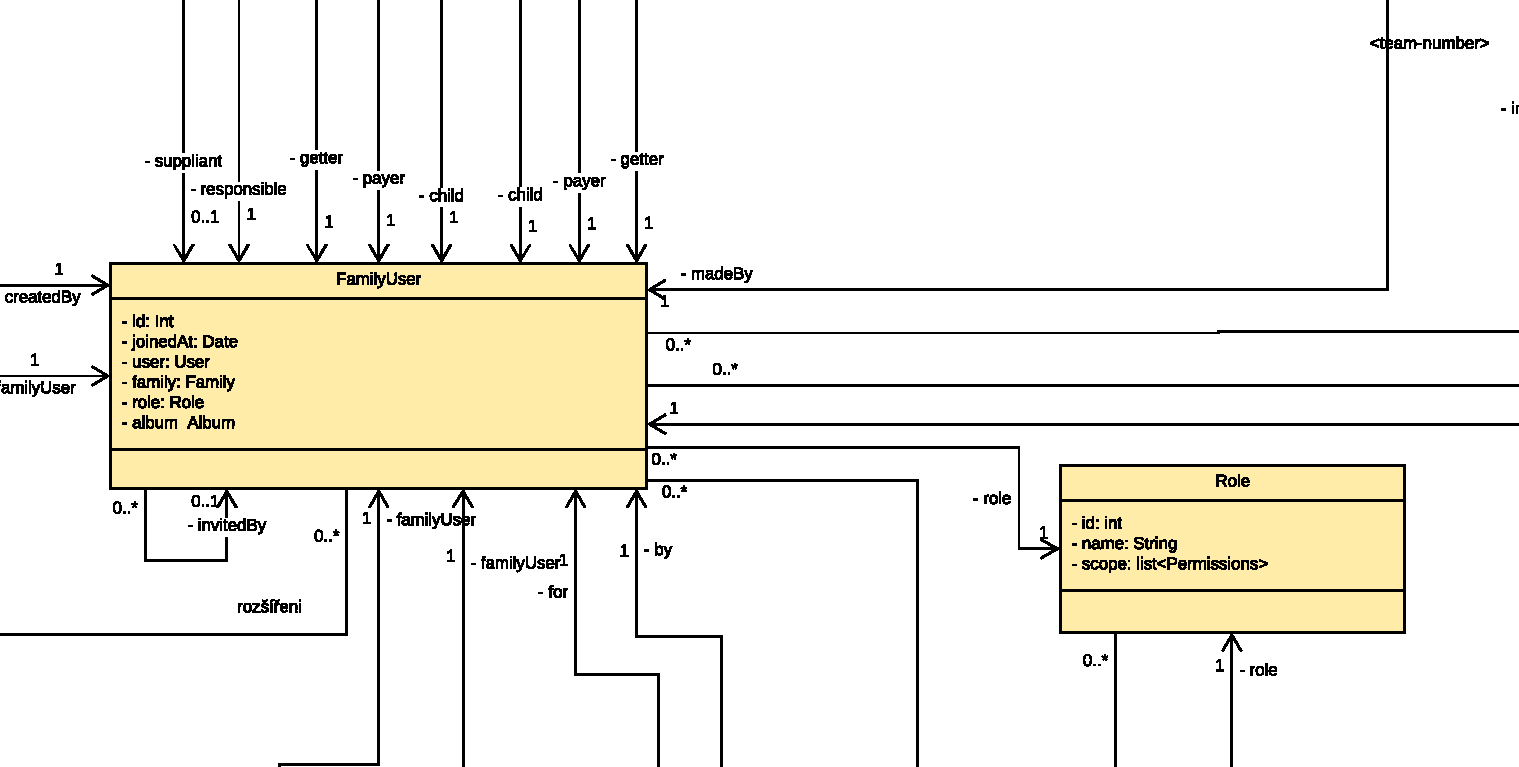
\includegraphics[width=1.0\textwidth]{pdfs/Role1}
	        \caption[Návrh \texttt{Role}]{Návrh entity \texttt{Role} podle doménového modelu z~předmětu BI-SP2}\label{image:Role1}
        \end{figure}
    % Navrh a Implementace 
    \begin{figure}\centering
	       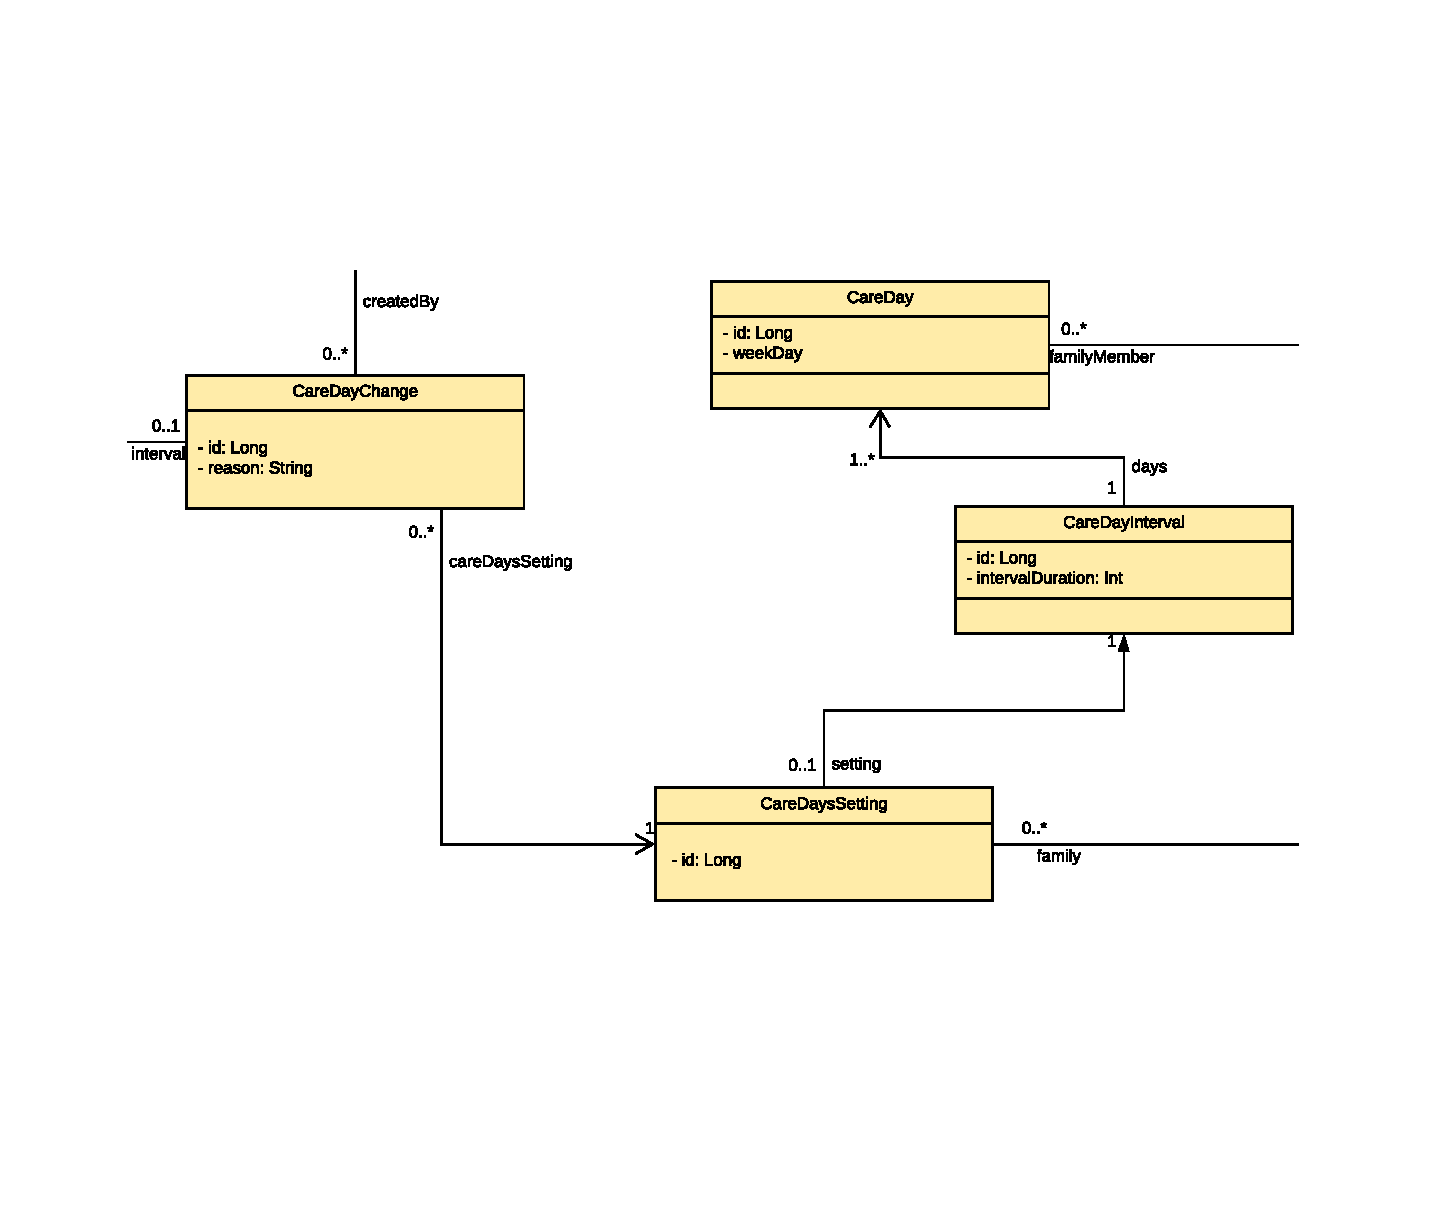
\includegraphics[angle=90, height=1.0\textheight]{pdfs/CareDays2}
	       \caption[Nový návrh pečovatelských dnů]{Nový návrh pečovatelských dnů}\label{image:caredays2}
        \end{figure}
    \begin{figure}\centering
        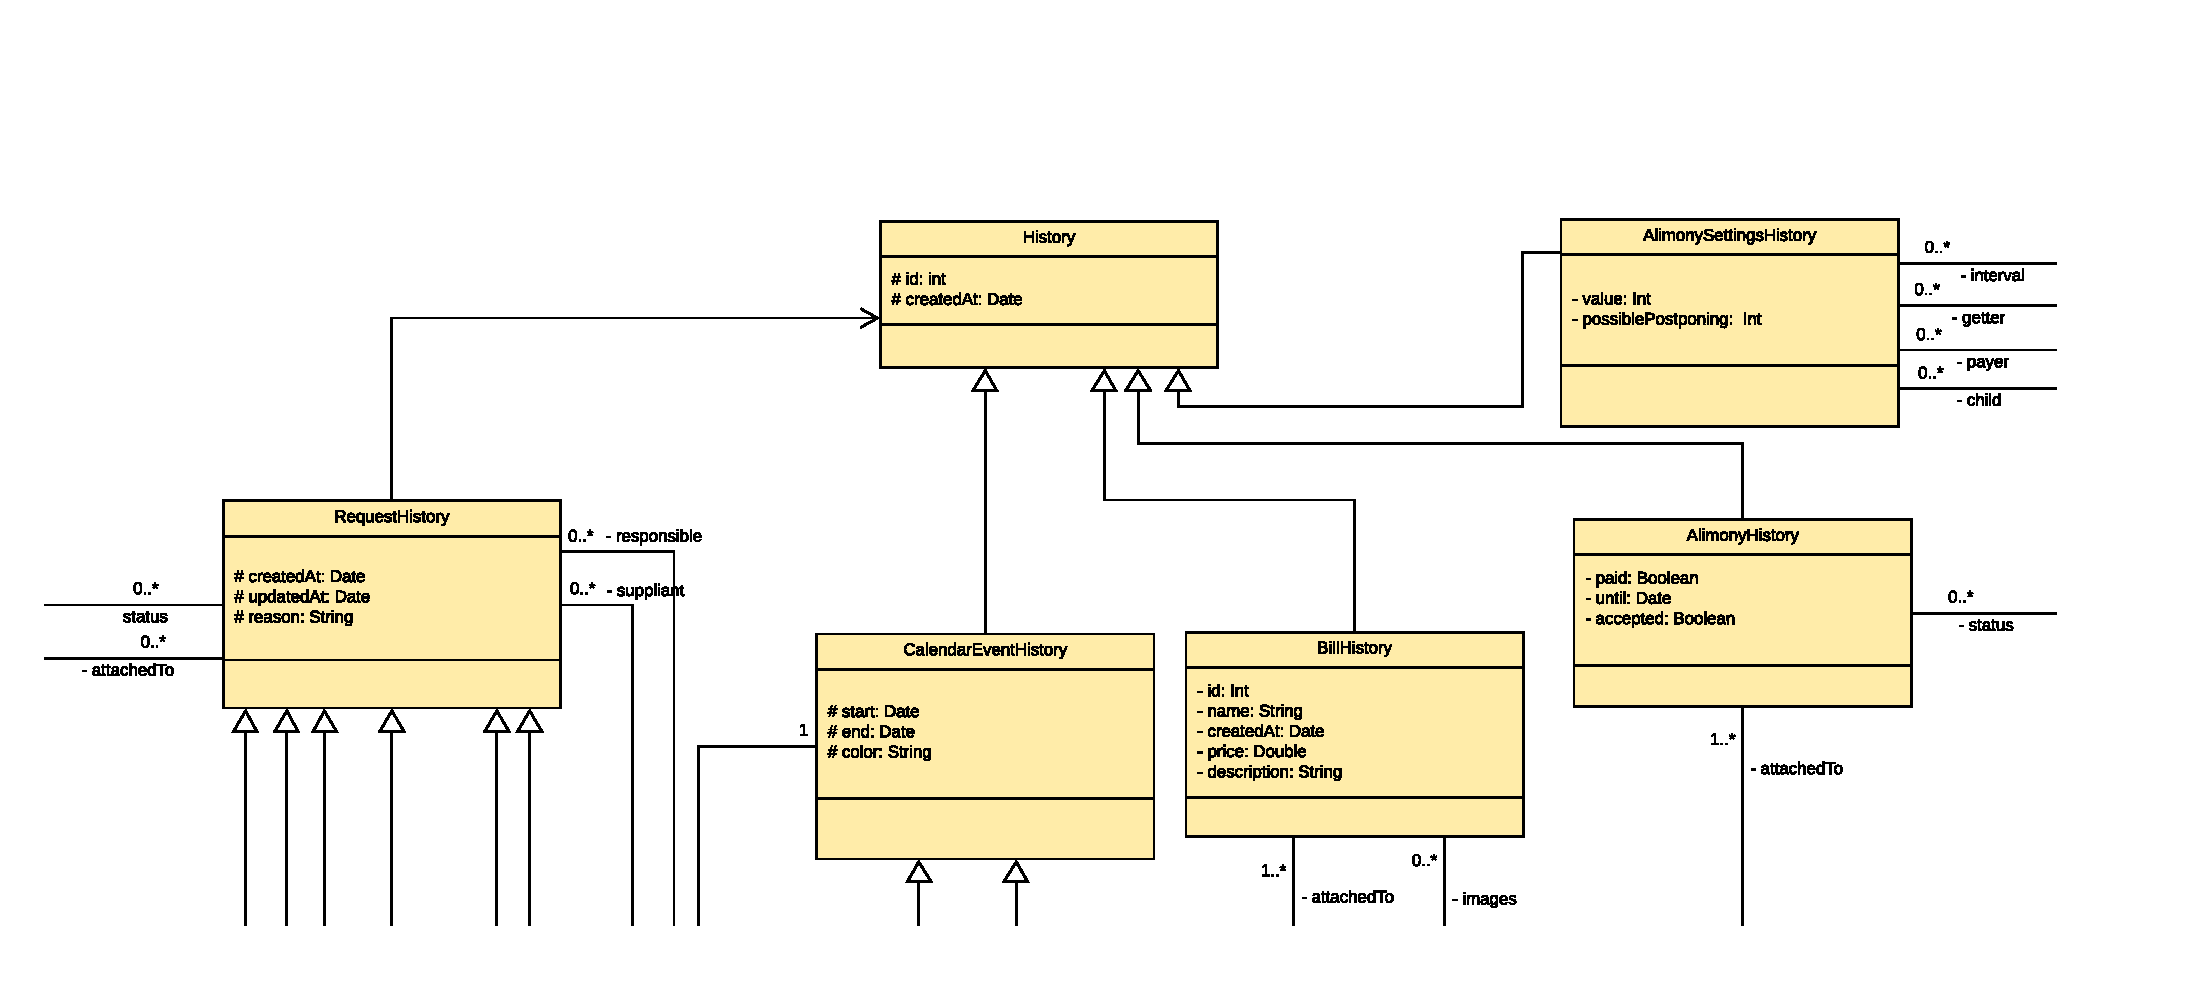
\includegraphics[angle=90, height=1.0\textheight]{pdfs/History1}
        \caption[Předešlý návrh entity \texttt{History}]{Předchozí návrh entity \texttt{History} podle doménového modelu z předmětu BI-SP2}\label{image:History1}
    \end{figure}
    \begin{figure}\centering
        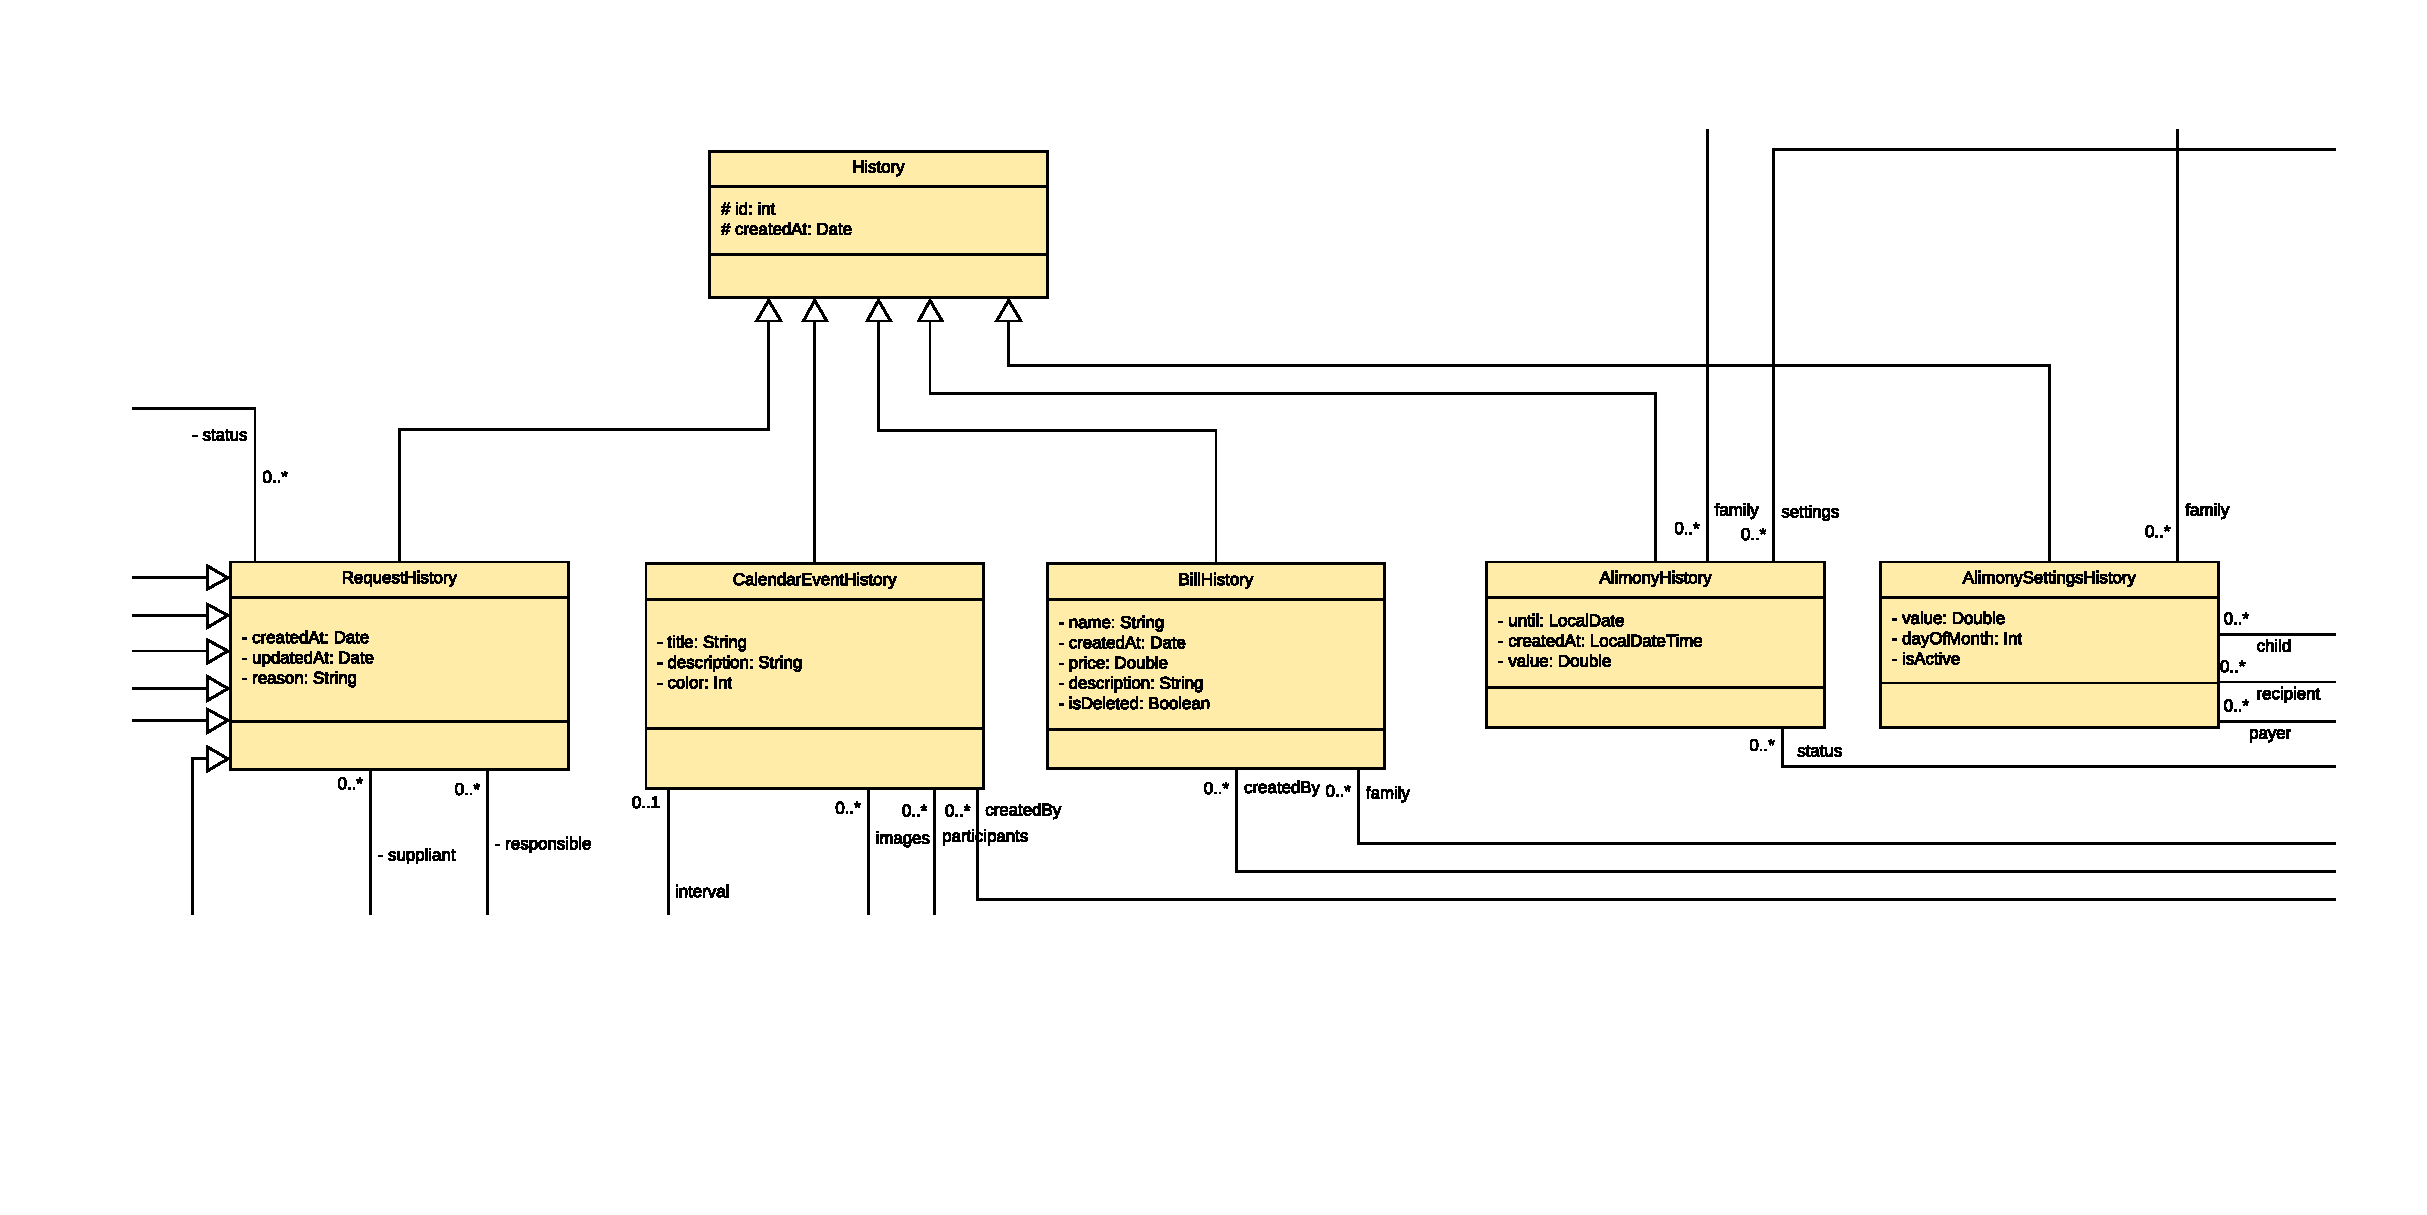
\includegraphics[angle=90, height=1.0\textheight]{pdfs/History1_2}
        \caption[Návrh entity \texttt{History} po změnách návrhu]{Návrh entity \texttt{History} po navržení změn pro entity, kterým patří příslušné entity historie}\label{image:History1_2}
    \end{figure}

